\documentclass[a4paper, 10pt]{paper}

\usepackage{listings}
\usepackage{amsmath}
\usepackage{geometry}
\usepackage{color}
\usepackage{natbib}
\usepackage{graphicx}
\usepackage{codedoc}

\title{StochBB -- Stochastic Building Blocks Manual}
\subtitle{Analyzing complex systems of dependent random variables}
\author{Hannes Matuschek}
\institution{Focus area \emph{Dynamics of complex systems},\\ University of Potdsam, Germany}


% Tiny macro to handle editorial notes as highligted text.
\newcommand{\todo}[1]{{\color{red}[TODO: #1]}}
% just highlight
\newcommand{\marked}[1]{{\color{red}#1}}
% highlight with comment
\newcommand{\comment}[2]{{\color{red}#1}\footnote{{\color{red}#2}}}
% to be removed
\newcommand{\remove}[1]{\color{red}\cancel{#1}}
% to be removed with comment
\newcommand{\removec}[2]{{\color{red}\cancel{#1}}\footnote{{\color{red}#2}}}


\setlength{\parindent}{0em}
\setlength{\parskip}{.8em}

% configure code display
\lstset{ %
  backgroundcolor=\color{white},         % choose the background color
  basicstyle=\footnotesize,              % size of fonts used for the code
  breaklines=true,                       % automatic line breaking only at whitespace
  captionpos=b,                          % sets the caption-position to bottom
  commentstyle=\color[rgb]{0.5,0.5,0.5}, % comment style
  keywordstyle=\color{blue},             % keyword style
  stringstyle=\color[rgb]{0.58,0,0.82}   % string literal style
}


\begin{document}

\maketitle
 
\section{Introduction} \label{sec:intro}
Frequently, complex systems are described in terms of stochastic processes, as the
underlying deterministic process is too complex to be modeled exactly or as the
process is indeed random. It is not always the random process itself that is of 
interest, but a derived quantity. For example, the distribution of waiting times until the
process reaches a certain state. In the field of cognition psychology, random processes are frequently used to
describe each processing stage in a chain of stages that leads to a response. The state of
each random process itself is usually not measurable but the total response time of all processing 
stages involved. Although each processing stage is modeled as a random process, the waiting-time
of a single stage is just a random variable and the complete system is then a system of dependent random 
variables.

StochBB is able to describe and analyze complex systems of dependent random variables
by combining simple ones (representing stages with a known waiting-time distribution) to
a complex system. For example, consider the following independent random variables
\begin{equation}
  X_1 \sim \Gamma(10, 100)\,, X_2 \sim \Gamma(20, 50)\text{ and } X_3 \sim \text{Exp}(0.01)\,,\nonumber
\end{equation}
which are described completely by their distribution. This means that the time, the
processing stage $X_1$ needs to complete is gamma-distributed with shape $k=10$ and scale
$\theta=100$. Analogously, the stages $X_2$ and $X_3$ are defined by their own waiting-time 
distribution.

From these basic building blocks, a more complex system can be assembled by
combining them. Using the example above, one may define a new processing stage that is a chain of
the stages $X_1,\dots,X_3$. This simple chain then describes the successive
processing of information entering the first stage described by $X_1$.
Once the first processing stage finished, its result gets forwarded to the second stage described
by $X_2$ and finally to the last stage described by $X_3$. The waiting time of the
complete chain is again a random variable that is the sum of all random variables,
or expressed mathematically
\begin{equation}
 Y = X_1 + X_2 + X_3\,. \nonumber
\end{equation}

SochBB determines the probability density function (PDF) or cumulative probability function
(CDF) of the waiting-time distribution of the process $Y$ analytically (as far as
possible) or resorts to a numeric method if the analytic approach fails. More over it provides an efficient
and correct sampler for the system of random variables.


\section{Representation and reductions of random variables}
Continuing the example above, please note that the sum of random variables commutes. Hence the
random variable $Y$ remains the same if defined as $Y = X_1 + X_3 + X_2$. Moreover, the 
distribution of the sum of $X_1$ and $X_3$ can be determined analytically as 
$X' = (X_1+X_3)\sim\Gamma(11,100)$. Hence the random variable $Y$ can now be expressed as 
$Y = X_2 + X'$, and only a single numeric convolution is necessary to obtain the PDF of the
random variable $Y$. 

StochBB implements several reductions of the system of random variables,
exploiting mathematical identities of random variables. To this end, it allows to obtain the PDFs and CDFs
of random variables efficiently.

\subsection{Affine transformations of random variables}
An affine transformation of the random variable $X$ has the form $Y = a\,X+b$, where $a\neq 0$
and $b$ are real values. Although affine transformations of random variables are not frequently
used directly in a system of random variables, they may appear as a result of other reductions
of the system. The PDF and CDF of the random variable $Y$ define above, are then simply 
\begin{equation}
 f_Y(y) = \frac{1}{a}f_X\left(\frac{y-b}{a}\right)\text{ and }
 F_Y(y) = F_X\left(\frac{y-b}{a}\right)\,. \nonumber
\end{equation}

Of course, an affine transformation of an affine transformed random variable $X$ is also a simple 
affine transformation of the random variable. Hence the following reduction is implemented
\begin{equation}
 c\,(a\,X+b)+d \longrightarrow (a\,c)\,X+(c\,b+d)\,.\nonumber
\end{equation}

\subsection{Sums of random variables}
Sums of random variables have been introduced briefly above and may represent a chain of processing
stages being triggered sequentially. The sum itself is a derived random variable that depends on all
mutually independent variables being summed up. The PDF of the sum $Y$ is then the convolution of all
PDFs of the summed variables. That is
\begin{align}
 Y &= \sum_{i=0}^NX_i\text{ where } X_i \sim f_i(x)\text{ mutually independent} \nonumber \\
 Y &\sim f_1(x) \ast \cdots \ast f_N(x)\,. \nonumber
\end{align}

The direct numerical convolution of the underlying distributions can be computationally expensive if the
number of PDFs is large. Assuming that all distributions are well supported on a common interval, however, 
allows for a fast numerical convolution by means of the FFT convolution. For the FFT convolution, all 
densities $f_i(x)$ are evaluated on a common regular gird and the evaluation of the convolution on that gird
can then be computed easily. This, however, requires that the grid is chosen such that all densities being
convoluted as well as the result are well supported on the chosen interval. Moreover, the grid must be fine 
enough to capture the details of all distributions. 

The numerical convolution, like any numerical approach, is only an approximation. Hence StochBB tries to perform
the convolutions analytically before resorting to the numerical approach. 

First all sums of random variables are flattened. That is, 
\begin{equation}
 \begin{array}{l}
  Y_1 = X_1 + X_2\\
  Y_2 = Y_1 + X_3 
 \end{array} \longrightarrow 
 \begin{array}{l}
  Y_1 = X_1 + X_2\\
  Y_2 = X_1 + X_2 + X_3 
 \end{array}\,. \nonumber
\end{equation}

Then, the distribution of the sum is derived. Here the following reductions are performed.
\begin{align}
 \delta(x-x_0)\ast U[a,b](x) &\longrightarrow U[a+x_0,b+x_0](x)\,, \nonumber \\
 \delta(x-x_0)\ast \phi(x; \mu, \sigma) &\longrightarrow \phi(x; \mu+x_0, \sigma)\,, \nonumber \\
 \phi(x; \mu_1, \sigma_1)\ast \phi(x; \mu_2, \sigma_2) &\longrightarrow 
   \phi(x; \mu_1+\mu_2, \sqrt{\sigma_1^2+\sigma_2^2}) \nonumber\,, \\
 \Gamma(x; k_1, \theta)\ast \Gamma(x; k_2, \theta) &\longrightarrow 
   \Gamma(x; k_1+k_2, \theta)\,, \nonumber
\end{align}
where $\delta(\cdot-x_0)$ is the delta distribution located at $x_0$, $U[a,b](\cdot)$ the uniform
distribution on the interval $[a,b]$, $\phi(\cdot; \mu, \sigma)$ the normal distribution with mean 
$\mu$ and standard deviation $\sigma$ and $\Gamma(\cdot; k, \theta)$ the gamma distribution with
shape $k$ and scale $\theta$.

\subsection{Minimum and maximum of random variables}
The minimum or maximum of some given random variables, e.g. $Y=\min\{X_1,X_2\}$ or 
$Y=\max\{X_1,X_2\}$ are them self random variables. These derived random variables can be used to
express the waiting time of a processing stage that consists of several independent processes being
performed in parallel (in contrast to sequential processes described by sums of random variables). 
If the processing stage is finished, once the first of the parallel processes is finished, the 
resulting waiting time is expressed by the minimum of the underlying random variables. If the stage
finishes once all underlying processes are finished, the resulting waiting time is described
by the maximum. 

If the two random variables $X_1$ and $X_2$ are distributed according to the (cumulative) distribution
functions $F_1(x)$ and $F_2(x)$, then the maximum of these two random variables $Y=\max\{X_1,X_2\}$
is distributed according to the probability function $F_Y(y)=F_1(y)\cdot F_2(y)$. Consequently, its PDF
is $f_Y(y)=f_1(y)\cdot F_2(y) + f_2(y)\cdot F_1(y)$, where $f_1(\cdot)$ and $f_2(\cdot)$ are the PDFs
of the random variables $X_1$ and $X_2$. Likewise, the CDF and PDF of the minimum can be expressed as
$F_Y(y)=1-(1-F_1(y))\cdot(1-F_2(y))$ and therefore $f_Y(y) = f_1(y)(1-F_2(y)) + f_2(y)(1-F_1(y))$.

For applying these equations to derive the CDF and PDFs of the minimum and maximum random variables, the 
underlying random variables must be independent. To achieve independence, where possible the following 
reductions are performed on maximum as well as minimum random variables.

Again, first maximum and minimum structures were flattened, for example
\begin{equation}
 \begin{array}{l}
  Y_1 = \max\{X_1,X_2\}\\
  Y_2 = \max\{Y_1,X_3\}
 \end{array} \longrightarrow
 \begin{array}{l}
  Y_1 = \max\{X_1,X_2\}\\
  Y_2 = \max\{X_1,X_2,X_3\}
 \end{array}\,, \nonumber
\end{equation}
then, possible common terms are collected like
\begin{equation}
 \max\{X_1 + X_2, X_3 + X_2\} \longrightarrow \max\{X_1,X_3\}+X_2\,. \nonumber
\end{equation}

This does not ensure independence of random variables, but decreases the complexity of
setting-up a complex system of random variables by resolving simple-structured 
dependencies between random variables.

\subsection{Mixture of random variables}
A mixture is the weighted sum of random variables
\begin{equation}
 Y = \frac{w_1X_1+\cdots+x_NX_N}{w_1+\cdots+w_N}\,, \nonumber
\end{equation}
where $w_i$ are positive weights, is also a random variable with the PDF
\begin{equation}
 f_Y(y) = \frac{w_1f_1(x)+\cdots+w_Nf_N(x)}{w_1+\cdots+w_N}\,,\nonumber
\end{equation}
where $f_i(\cdot)$ is the PDF of the i-th random variable $X_i$. The CDF of the
mixture is obtained analogously. A mixture can be used to describe a random 
path-selection in a system of processing stages. 

\subsection{Compound random variables}
The most complex derived random-variable type is the compound random variable. That is a random variable
$X$ distributed according to a parametric distribution $X\sim f_{X|A}(x;A)$ with parameter $A$. $A$, however, 
is a random variable by itself with its own distribution $A\sim g(a)$. The distribution of the compound 
random variable $X$ is then obtained by marginalizing the parameter of the PDF $f_{X|A}(\cdot;a)$ as 
\begin{equation}
 f_X(x) = \int f_{X|A}(x;a)\,g(a)\,da\,,\nonumber
\end{equation}
and the CDF is obtained analogously as
\begin{equation}
 F_X(x) = \int F_{X|A}(x;a)\,g(a)\,da\,.\nonumber
\end{equation}

StochBB determines the PDF and CDF of $X$ by performing the integral numerically using a similar \emph{trick}
as for the convolution of PDFs. Here the parameter distribution is evaluated on the same grid as the distribution
of the random variable $X$ itself, allowing to determine the approximate PDF of the compound. This, however, requires 
that both distributions, the distribution of the parameter and the distribution of the variable itself have similar 
scales. This assumption is not always met. If violated, the resulting approximation might be bad.


\section{Application programming interface} \label{sec:api}
The application programming interface (API, see also \cite{stochbbapi}) allows to assemble processes
programmatically in C++.
All API classes are derived from the \class{Container} class which is an essential part of the
memory management system used by StochBB. Usually the C++ programmer needs to keep track of all
objects still in use and is responsible to free unneeded objects to avoid memory leaks. This can
be a difficult takes when dealing with complex structured objects cross referencing each other.
To ease the usage of StochBB, a \emph{mark and sweep} garbage collector is implemented which keeps track
of all objects being directly or indirectly reachable and freeing all unreachable objects. For
this memory management system to work, it is necessary to treat all container objects like values
although they represent references to objects allocated on the heap.

The central class of StochBB is \class{Var}, representing a random variable. This could be a
simple random variable having a specified distribution (see \class{AtomicVar}) or a random
variable that is derived from others like \class{Chain}, \class{Minimum}, \class{Maximum} or
\class{Mixture}. All random variables have probability density function attached. They can be accessed
using the \method{Var}{density} method which returns a \class{Density} object.

All \class{Density} objects have two methods, \method{Density}{eval} evaluating the probability
density function and \method{Density}{evalCDF} evaluating the cumulative density or probability
function. Assembling a system of random variables and evaluate their PDFs or CDFs is straight
forward. Sampling, however, is not that trivial and is described below in some detail.

\subsection{Assembling a system of random variables}
In a first step, one may define a new gamma-distributed random variable with shape $k=10$
and scale $\theta=100$ as
\begin{lstlisting}[language=C++]
 #include <stochbb/api.h>
 using namespace sbb;
 
 // [...]
 
 Var X1 = sbb::gamma(10, 100);
\end{lstlisting}

Its PDF can then be evaluated as on a regular grid in $[0,1000)$ with $1000$ grid points as
\begin{lstlisting}[language=C++]
 // [...]
 
 Eigen::VectorXd pdf(1000);
 X1.density().eval(0, 1000, pdf);
\end{lstlisting}

The result of the evaluation is stored into the vector \code{pdf}. There are only very few basic
or atomic random-variable types defined in StochBB:

\begin{tabular}{l|l|l}
 Constructor & Parameters & Process description \\ \hline
 \function{sbb::delta} & \code{delay} & A constant delay or a process with a fixed waiting time. \\
 \function{sbb::unif} & \code{a}, \code{b} & A process with a uniform-distributed waiting time. \\
 \function{sbb::norm} & \code{mu}, \code{sigma} & A process with a normal-distributed waiting. \\
 \function{sbb::gamma} & \code{k}, \code{theta} & A process with a gamma-distributed waiting time. \\
\end{tabular}

More complex processes can be derived by combining these atomic random variables or as special cases of them.

\subsubsection{Affine transformation of random variables}
An affine transformation of the random variable $X$ is of the form $a\,X+b$, where $a\neq 0$ and $b$ are
real values. An affine transformation can be obtained using the overloaded * and + operators or using the
\function{affine} function. For example, the code
\begin{lstlisting}[language=C++]
 #include <stochbb/api.h>
 using namespace sbb;
 
 // [...]
 
 Var X = sbb::gamma(10, 100);
 Var Y = 3*X + 1;
\end{lstlisting}
constructs a random variable \code{Y} being an affine transformed of the random variable \code{X}.

\subsubsection{Sums of random variables}
The most basic derived random variable is a \class{Chain}. This type represents the \emph{chaining} of
random processes. Such a chain can be constructed using the overloaded \code{+} operator
or the \function{chain} function. For example
\begin{lstlisting}[language=C++]
 #include <stochbb/api.hh>
 using namespace sbb;

 // [...]

 Var X1 = sbb::gamma(10,100);
 Var X2 = sbb::gamma(20, 50);
 Var Y = X1 + X2;
\end{lstlisting}

\subsubsection{Minimum and Maximum of random variables}
Another simple derived random variable is the \class{Maximum} or \class{Minimum} class. As the
names suggest, they represent the maximum or minimum of a set of random variables. They can be
created using the overloaded standard library function \function{std::min} and \function{std::max} or the
\function{minimum} and \function{maximum} functions. The latter take a vector of random variables.
\begin{lstlisting}[language=C++]
 #include <stochbb/api.hh>
 using namespace sbb;

 // [...]

 Var X1 = sbb::gamma(10,100);
 Var X2 = sbb::gamma(20, 50);
 Var Y = std::max(X1, X2);
\end{lstlisting}

\subsubsection{Mixtures of random variables}
Similar to the \class{Minimum} or \class{Maximum}, a mixture of random variables can be
constructed using the \function{mix} function. This function takes a vector of weights and a vector
of corresponding random variables. Such a mixture can be considered as a random process which
randomly selects the outcome of a set of other random processes, where the probability of
selecting a specific process is given by the relative weight assigned to each process.
\begin{lstlisting}[language=C++]
 #include <stochbb/api.hh>
 using namespace sbb;

 // [...]

 Var X1 = sbb::gamma(10,100);
 Var X2 = sbb::gamma(20, 50);
 // Assemble vector of variables
 std::vector<Var> vars; var.push_back(X1), vars.push_back(X2);
 // Assemble vector of weights
 std::vector<double> weights; var.push_back(1), vars.push_back(2);
 // Construct mixture
 Var Y = sbb::mix(weights, vars);
\end{lstlisting}

In the example above, the random process $Y$ will select the outcome of $X_1$ with
a probability of $\frac{1}{3}$ and the outcome of $X_2$ with probability
$\frac{2}{3}$.

\subsubsection{Compound random variables}
An important class of derived random processes are compound processes. There the parameters of the
distribution of a random variable are themselves random variables. That is
\begin{equation}
 X \sim f(x|A)\,,\quad A \sim g(a|\theta)\,, \nonumber
\end{equation}
where the random variable $X$ is distributed as $f(x|A)$, parametrized by $A$,
where $A$ itself is a random variable distributed as $g(a|\theta)$, parametrized by
$\theta$. 

Compound random variables are created using the same factory function like the atomic random variable
types. In contrast to the atomic random variables, the factory functions take random variables as 
parameters instead of constant values.
\begin{lstlisting}[language=C++]
 #include <stochbb/api.hh>
 using namespace sbb;
 
 // [...]
 
 Var mu = sbb::gamma(10,100);
 Var cnorm = sbb::norm(mu, 10);
\end{lstlisting}
instantiates a compound-normal distributed random variable, where the mean is gamma distributed
while the standard deviation is fixed.

\subsection{Sampling several dependent random variables}
As mentioned above, sampling from a complex process efficiently is not trivial. First of all, is
must be ensured that all atomic random variables are samples only once. Otherwise, two dependent
random variables may be sampled as independent. Moreover, the results of derived random variables
should be cached for efficiency. 

StochBB provides a separate class that implements a proper
sampler for a system of random variables, the \class{ExactSampler} class. This class allows to
sample from several possibly dependent random variables simultaneously. Upon construction, the
set of random variables to sample is specified. A sample from these random variables can then be
obtained by the \method{ExactSampler}{sample} method.
\begin{lstlisting}[language=C++]
 #include <stochbb/api.hh>
 using namespace sbb;

 // [...]

 Var X1 = sbb::gamma(10,100);
 Var X2 = sbb::gamma(20, 50);
 Var Y = std::min(X1, X2);
 // Construct sampler
 ExactSampler sampler(X1, X2, Y);
 // Get 1000 samples
 Eigen::MatrixXd samples(3, 1000);
 sampler.sample(samples);
\end{lstlisting}

The \method{ExactSampler}{sample} method takes a single \class{Eigen::Matrix} where each column
represents the random variable given to the constructor and each row an independent sample from
the system.

For very large systems, sampling may get slow. Particularly if one is only interested
in the marginal distribution of single random variables. For these cases a approximate sampler
for single random variables is provided, the \class{MarginalSampler}. This sampler uses an
approximation of the inverse of the cumulative distribution function of a random variable
to draw samples.
\begin{lstlisting}[language=C++]
 #include <stochbb/api.hh>
 using namespace sbb;

 // [...]

 Var X1 = sbb::gamma(10,100);
 Var X2 = sbb::gamma(20, 50);
 Var Y = std::min(X1, X2);
 // Sample from Y on [0,500] in 1000 steps
 MarginalSampler sampler(Y, 0, 500, 1000);
 // Get 1000 samples
 Eigen::VectorXd samples(1000);
 sampler.sample(samples);
\end{lstlisting}

In this example, a \class{MarginalSampler} is constructed for the random variable \code{Y}. Using an
approximation of its CDF on the interval $[0,500)$ using $1000$ steps. Then, the
\method{MarginalSampler}{sample} method is used to obtain $1000$ independent samples.


\section{Process \& simulation description in XML} \label{sec:xml}
In contrast to the application programming interface (see Section \ref{sec:api}, above), 
complex processes can also be defined in XML and analyzed using the
StochBB command line tool (see Section \ref{sec:cli}, below). A single XML file defines a 
\class{Simulation}, a simple collection of random variables together with the specification which
variables as used for the output. For example the XML code
\begin{lstlisting}[language=XML]
 <?xml version="1.0"?>
 <simulation xmlns="http://hmatuschek.github.io/stochbb/simulation-0.0.dtd"
             xmlns:m="http://www.w3.org/1998/Math/MathML">

  <var type="gamma" id="gamma">
   <param name="k"> <m:cn>5</m:cn> </param>
   <param name="theta"> <m:cn>30</m:cn> </param>
  </var>

  <output from="0" to="100">
   <var ref="gamma"/>
  </output>

 </simulation>
\end{lstlisting}
specifies a trivial simulation.

Here a single gamma-distributed random variable is defined.
It gets the identifier \code{gamma} assigned. With this identifier, it is possible to refer to the random
variable later. The \code{type} attribute specifies the type of the random variable. Here the
build-in type \code{gamma} is used, specifying a gamma-distributed random variable. The shape and
scale parameters, \code{k} and \code{theta}, are specified using the \code{param} elements. 
The \code{name} attribute of each \code{param} element specified the name of the parameter while 
its value is given as an MathML child element of the \code{param} element.

Finally, the \code{output} element specifies which random variables are used for output. Each child
element of the \code{output} element specifies one variable. Either by referencing a previously defined
random variable or by specifying the random variable directly. For example,
\begin{lstlisting}[language=XML]
 <?xml version="1.0"?>
 <simulation xmlns="http://hmatuschek.github.io/stochbb/simulation-0.0.dtd"
             xmlns:m="http://www.w3.org/1998/Math/MathML">

  <output from="0" to="100">
   <var type="gamma">
    <param name="k"> <m:cn>5</m:cn> </param>
    <param name="theta"> <m:cn>30</m:cn> </param>
   </var>
  </output>

 </simulation>
\end{lstlisting}
is fully equivalent to the previous example.

\subsection{Build-in random variables}
There are only very few build-in random variable types. They can be divided into two groups:
\emph{atomic} and \emph{derived} random variables.

\subsubsection{Atomic random variables}
Atomic random variables are random variables which follow a specific
distribution and are independent from any other random variable defined.

\begin{tabular}{l|l|l}
 Type & Parameters & Process description \\ \hline
 \code{delta} & \code{delay} & A constant delay or a process with a fixed waiting time. \\
 \code{uniform} & \code{a}, \code{b} & A process with a uniform-distributed waiting time. \\
 \code{normal} & \code{mu}, \code{sigma} & A process with a normal-distributed waiting. \\
 \code{gamma} & \code{k}, \code{theta} & A process with a gamma-distributed waiting time.
\end{tabular}

Beside these atomic random variables, there are derived random variables which depend on other
random variables. Hence they usually do not take simple parameters as arguments but other 
random variables.

\subsubsection{Chains of random variables}
One of the most important derived random variable is a chain. A chain can be defined as
\begin{lstlisting}[language=XML]
 <var type="chain">
  <var ref="X1"/> <var ref="X2"/> <var ref="X2"/>
 </var>
\end{lstlisting}

Here the random variable \code{X1}, \code{X2} and \code{X3} are chained. Mathematically,
the waiting time of the chain is simply the sum of the waiting times of the random variables
\code{X1}--\code{X3}.

\subsubsection{Maximum of random variables}
Another derived random variable is the \code{maximum} type. This type can be interpreted as a
processes that waits until all referred parallel processes are completed hence the waiting time
of
\begin{lstlisting}[language=XML]
 <var type="maximum">
  <var ref="X1"/> <var ref="X2"/> <var ref="X2"/>
 </var>
\end{lstlisting}
is just the maximum of the random variables \code{X1}--\code{X3}.

\subsubsection{Minimum of random variables}
Likewise, the \code{minimum} derived random variable is simply the minimum of the referred random
variables and represents the waiting time of the fastest parallel processes \code{X1}--\code{X3}:
\begin{lstlisting}[language=XML]
 <var type="minimum">
  <var ref="X1"/> <var ref="X2"/> <var ref="X2"/>
 </var>
\end{lstlisting}

\subsubsection{Mixture of random variables}
The mixture of random variables is defined using the \code{mixture} variable type with a list of
weight-variable pairs. For example
\begin{lstlisting}[language=XML]
 <var type="mixture">
  <weight> <m:cn>1</m:cn> <var ref="X1"/> </weight>
  <weight> <m:cn>2</m:cn> <var ref="X2"/> </weight>
  <weight> <m:cn>1</m:cn> <var ref="X3"/> </weight>
 </var>
\end{lstlisting}

\subsubsection{Compound random variables} 
A compound random variable $Y$ has a distribution $f_{Y|A}(y|A)$ where the parameter $A$ is a random
variable too, with its own distribution $A~g()$. In XML a compound is specified using the 
\code{compound} type by specifying the base type of the distribution using the \code{base} attribute.
Instead of simple parameters, the parameters of an compound are specified as random variables. 
For example, the code
\begin{lstlisting}[language=XML]
 <var id="mu" ...>
  [ ... ]
 </var>
 <var id="sigma" ...>
  [ ... ]
 </var>
 
 <var type="compound" base="normal">
  <param name="mu"> <var ref="mu"/> </param>
  <param name="sigma"> <var ref="sigma"/> </param>
 </var>
\end{lstlisting}
defines a compound-normal distributed random variable where its mean is distributed like the random 
variable \code{mu} and its standard deviation like \code{sigma}. Of course these parameter random 
variables have to be defined earlier.

\subsection{User defined random-variable types}
The limited number of build-in random-variable types would turn the definition of complex stationary random
processes difficult. Hence it is possible to define new types derived from the build-in ones. For example,
the code 
\begin{lstlisting}[language=XML]
 <define id="exp">
  <param id="lambda"/>

  <var type="gamma" id="exp">
   <param name="k"><m:cn>1</m:cn></param>
   <param name="theta">
    <m:apply>
     <m:divide/>
     <m:cn>1</m:cn>
     <m:ci>lambda</m:ci>
    </m:apply>
   </param>
  </var>
 </define>
\end{lstlisting}
defines a new type \code{exp} as a special case of the Gamma distribution as
$\text{Exp}(\lambda) = \Gamma(1,\lambda^{-1})$. The \code{define} tag takes an \code{id} 
attribute specifying the new type identifier. Then, one ore more \code{param} elements are
used to specify the parameters of the new type. 
Here only one parameter named \code{lambda} is defined. Finally a random variable with the same
identifier as the type name is defined which implements the new random variable type.

A more complex example might be
\begin{lstlisting}[language=XML]
 <define id="exgauss">
  <param id="lambda">
  <param id="mu"/>
  <param id="sigma"/>

  <var type="gamma" id="ex">
   <param name="k"><m:cn>1</m:cn></param>
   <param name="theta">
    <m:apply>
     <m:divide/>
     <m:cn>1</m:cn>
     <m:ci>lambda</m:ci>
    </m:apply>
   </param>
  </var>

  <var type="normal" id="gauss">
   <param name="mu"> <m:ci>mu</m:ci> </param>
   <param name="sigma"> <m:ci>sigma</m:ci> </param>
  </var>

  <var type="chain" id="exgauss">
    <var ref="ex"/> <var ref="gauss"/>
  </var>
 </define>
\end{lstlisting}

This defines a new random-variable type with an exponentially modified Gaussian (Ex-Gauss) 
distribution by chaining an exponential- (defined here as a special case of the Gamma 
distribution) and a Gaussian-distributed random variable. This new type can then be used
to instantiate Ex-Gauss-distributed random variables as
\begin{lstlisting}[language=XML]
 <var type="exgauss">
  <param name="lambda"> <m:cn>10</m:cn> </param>
  <param name="mu"> <m:cn>20</m:cn> </param>
  <param name="sigma"> <m:cn>10</m:cn> </param>
 </var>
\end{lstlisting}

\subsection{Modules}
Some of the aforementioned user defined random variable types may be reused in several
simulations. For these cases it is convenient to export these definitions into separate files
and load them when needed. These files are called modules and form simple collections of
variable type definitions. For example a module defining the an exponential distributed 
random variable could be implemented as
\begin{lstlisting}[language=XML]
 <?xml version="1.0"?>
 <module xmlns="http://hmatuschek.github.io/stochbb/module-0.0.dtd"
             xmlns:m="http://www.w3.org/1998/Math/MathML">

  <define id="exp">
   <param id="lambda"/>

   <var type="gamma" id="exp">
    <param name="k"><m:cn>1</m:cn></param>
    <param name="theta">
     <m:apply>
      <m:divide/>
      <m:cn>1</m:cn>
      <m:ci>lambda</m:ci>
     </m:apply>
    </param>
   </var>
  </define>

 </module>
\end{lstlisting}

Within the body of the module, the user-defined types can be specified. Such a module can then
be loaded using the \code{load} tag within a simulation or other modules like
\begin{lstlisting}[language=XML]
 <?xml version="1.0"?>
 <simulation xmlns="http://hmatuschek.github.io/stochbb/simulation-0.0.dtd"
             xmlns:m="http://www.w3.org/1998/Math/MathML">

  <load>exp.xml</load>

  <output ...>
   [ ... ]
  </output>
 </simulation>
\end{lstlisting}

With this XML language, it is possible to specify complex systems of random variables that can be analyzed 
using the \code{stochbb} command line tool described in the next section.

\section{Command line interface} \label{sec:cli}
The StochBB installation comes with a command line tool. With this tool, a process definition
in XML (see Section \ref{sec:xml}) can be analyzed. The results are returned as CSV or they can be plotted
directly.

\subsection{Synopsis}
\begin{lstlisting}
 stochbb [OPTIONS] [CMD] INPUTFILE [OUTPUT OPTIONS]
\end{lstlisting}

\subsubsection{Options}
\begin{tabular}{p{.3\textwidth}p{.6\textwidth}}
 \code{--help} & Prints a short help string and exits. \\
 \code{--version} & Prints the version string and exits. \\
 \code{--log-debug} &Prints debug messages to stderr. By default, only warnings and error messages
  are printed to stderr. 
\end{tabular}

\subsubsection{Commands}
\begin{tabular}{p{.3\textwidth}p{.6\textwidth}}
 \code{pdf} & Specifies to evaluate the PDF of the variables selected in the \code{INPUTFILE} (default). \\
 \code{cdf} & Specifies to evaluate the CDF instead of the PDF of the variables selected in the
  \code{INPUTFILE}. \\
 \code{sample} & Samples from the variables selected in the \code{INPUTFILE}.
\end{tabular}

\subsubsection{Output options}
\begin{tabular}{p{.3\textwidth}p{.6\textwidth}}
 \code{--plot} & Plots the marginal PDFs or CDFs of the output variables specified in the \code{INPUTFILE}. \\
 \code{--csv=FILENAME} & Writes the PDFs or CDFs of the output variables specified in the \code{INPUTFILE}
  to \code{FILENAME}.
\end{tabular}

By default, the results (evaluated PDFs, CDFs or drawn samples) are printed to stdout, allowing for the direct usage 
of the results by other command line tools.

\subsection{Examples}
The following examples use the following system definition stored in a file name \code{example.xml}:
\begin{lstlisting}[language=XML]
<?xml version="1.0"?>

<simulation xmlns="http://hmatuschek.github.io/stochbb/simulation-0.0.dtd"
            xmlns:m="http://www.w3.org/1998/Math/MathML">

 <load>exp.xml</load>

 <var type="exp" id="X1">
  <param name="lambda"> <m:cn>0.01</m:cn> </param>
 </var>

 <var type="exp" id="X2">
  <param name="lambda"> <m:cn>0.02</m:cn> </param>
 </var>

 <var type="maximum" id="max" name="max(X1,X2)">
  <var ref="X1"/> <var ref="X2"/>
 </var>

 <output from="0" to="300" steps="1000">
  <var ref="X1"/> <var ref="X2"/> <var ref="max"/>
 </output>
</simulation>
\end{lstlisting}

Using this example system, the following call plots the PDFs of the random variables \code{X1}, \code{X2} and \code{max} defined in XML above
\begin{lstlisting}
 stochbb pdf example.xml --plot
\end{lstlisting}
The resulting plot is shown in Figure \ref{fig:exampleplot1}.	

\begin{figure}
 \centering
  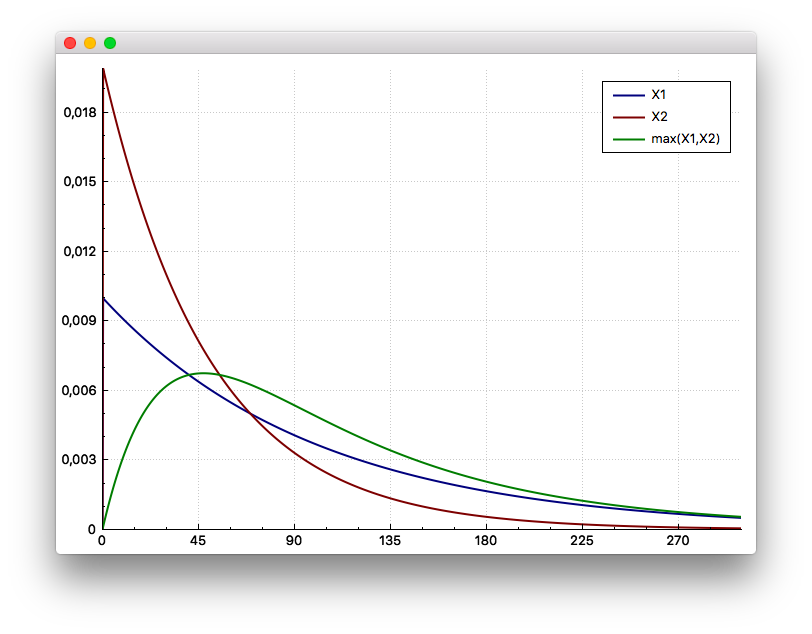
\includegraphics[width=0.7\textwidth]{exampleplot1.png}
  \caption{Plot of the marginal PDFs of the random variables $X_1\sim \text{Exp}(0.01)$, $X_2\sim \text{Exp}(0.02)$ and 
	$max = \max\{X_1,X_2\}$ as generated by the \code{stochbb} command line tool.} \label{fig:exampleplot1}
\end{figure}

The same PDF can be stored as CSV in \code{output.csv} by calling
\begin{lstlisting}
 stochbb pdf example.xml --csv=output.csv
\end{lstlisting}
or printed to stdout by calling 
\begin{lstlisting}
 sotchbb pdf example.xml
\end{lstlisting}

Finally, the call
\begin{lstlisting}
 sotchbb sample example.xml --csv=output.csv
\end{lstlisting}
draws 1000 samples of the random variables \code{X1}, \code{X2} and \code{max} defined in XML above.


\bibliographystyle{plain}
\bibliography{references}


\clearpage
\appendix
\section{Brief API Documentation} \label{sec::apidoc}
Beside the brief API discussion above (see Section \ref{sec:api}) this appendix provides some details on the available classes and 
functions defined as the application programming interface of StochBB. You can find a complete API reference including the documentation
of internal used object at \citep{stochbbapi}.

\begin{deffunc}{sbb::delta}{\class{Var}}{double value}	
 Constructs a new delta-distributed random variable located at \code{value}, that is $\delta(x-x_0)$.
\end{deffunc}

\begin{deffunc}{sbb::unif}{\class{Var}}{double a, double b}	
Constructs a new uniform-distributed random variable on the interval $[a,b]$, that is $\text{U}[a,b](x)$.
\end{deffunc}

\begin{deffunc}{sbb::norm}{\class{Var}}{double mu, double sigma}
Constructs a new normal-distributed random variable with mean \code{mu} and 
standard deviation \code{sigma} , that is $\phi(x;\mu, \sigma)$.
\end{deffunc}

\begin{deffunc*}{sbb::norm}{\class{Var}}{const \class{Var}\& mu, const \class{Var}\& sigma}
Constructs a new compound-normal-distributed random variable with mean \code{mu} and 
standard deviation \code{sigma} being random variables too.
\end{deffunc*}

\begin{deffunc}{sbb::gamma}{\class{Var}}{double k, double theta}
Constructs a new gamma or compound-gamma-distributed random variable with shape \code{k} and 
scale \code{theta} , that is $\Gamma(x; k, \theta)$.
\end{deffunc}

\begin{deffunc*}{sbb::gamma}{\class{Var}}{const \class{Var}\& k, const \class{Var}\& theta}
Constructs a new gamma or compound-gamma-distributed random variable with shape \code{k} and 
scale \code{theta} begin random variables too.
\end{deffunc*}

\begin{deffunc}{sbb::affine}{\class{Var}}{const \class{Var}\& X, double a, double b}
Constructs an affine transformed random variable from the given one as $Y = a\,X+b$.
\end{deffunc}

\begin{deffunc}{sbb::chain}{\class{Var}}{const std::vector<\class{Var}>\& variables}
Constructs a chain of several random variables as $Y = \sum_i X_i$. 
\end{deffunc}

\begin{deffunc}{sbb::maximum}{\class{Var}}{const std::vector<\class{Var}>\& variables}
Constructs a maximum random variable, a variable that represents the maximum of several other random variables as $Y = \max\{X_1,...,X_N\}$.
\end{deffunc}

\begin{deffunc}{sbb::minimum}{\class{Var}}{const std::vector<\class{Var}>\& variables}
Constructs a minimum random variable, a variable that represents the minimum of several other random variables as $Y = \min\{X_1,...,X_N\}$.
\end{deffunc}


\defclass{Container}
Base class of all container object holding references to managed objects. This class is an essential part of the internal memory 
management system. All classes of the API are derived from this class.

\begin{classsyn}{Container}{}
Constructs an empty container.
\end{classsyn}

\begin{defmeth}{Container}{isNull}{bool}{}
Returns \code{true} if the container is empty, that is if the container does not refer to an actual object.
\end{defmeth}

\begin{defmeth}{Container}{is<Type>}{bool}{}
Returns \code{true} if the container holds a reference to an object of type \code{Type} and \code{false} otherwise. 
This template method can be used to test a container before casting it with \method{Container}{as<Type>}.
\end{defmeth}

\begin{defmeth}{Container}{is<Type>}{Type}{}
Casts the container to the type \code{Type}. Returns an empty container if cast fails, e.g. if the reference held by the 
container cannot be casted to the given type.
\end{defmeth}


\defclassex{Var}{Container}
Base class of all random variables. All random variables have a probability density function assigned which can be accessed
using \method{Var}{density} method.

\begin{classsyn}{Var}{} 
Constructs an empty variable container.
\end{classsyn}

\begin{defmeth}{Var}{density}{\class{Density}}{}
Returns the density of the random variable.
\end{defmeth}

\begin{defmeth}{Var}{dependsOn}{bool}{const Var\& var}
Returns \code{true} if the random variable depends on the given variable \code{var}.
\end{defmeth}

\begin{defmeth}{Var}{mutuallyIndep}{bool}{const Var\& var}
Returns \code{true} if the random variable and the given variable are mutually independent.
\end{defmeth}


\defclassex{Density}{Container}
Base class of all probability density functions (PDFs).

\begin{defmeth}{Density}{eval}{void}{double min, double max, Eigen::VectorXd\& out}
Evaluates the PDF on a regular grid in $[min, max)$ using the same number of grid points as the number
of elements in \code{out}.
\end{defmeth}
 
\begin{defmeth}{Density}{evalCDF}{void}{double min, double max, Eigen::VectorXd\& out}
Evaluates the cumulative probability function (CDF) on a regular grid in $[min, max)$ using the same number
of grid points as the number of elements in \code{out}.
\end{defmeth}


\defclassex{DerivedVar}{Var}
Base class of all derived random variables, that are random variables which are defined as functions of other random 
variables.

\begin{defmeth}{DerivedVar}{numVariables}{size\_t}{}
Returns the number of variables the derived variable depends on.
\end{defmeth}

\begin{defmeth}{DerivedVar}{numVariables}{\class{Var}}{size\_t i}
Returns the \code{i}-th random variable the derived variable depends on.
\end{defmeth}


\defclass{AffineTafo}{DerivedVar}
This class represents an affine transformed random variable, that is $Y = a\,X+b$. This class does not provide a
public constructor, use the \function{sbb::affine} function to construct an affine transformation.

\begin{defmeth}{AffineTrafo}{scale}{double}{}
 Returns the scale of the transform, a.k.a. $a$.
\end{defmeth}

\begin{defmeth}{AffineTrafo}{shift}{double}{}
 Returns the shift of the transform, a.k.a. $b$.
\end{defmeth}


\defclass{Chain}{DerivedVar}
Implements the sum of the independent random variables $X_i, i=1,\dots,N$, $Y = \sum_i X_i$.

\begin{classsyn}{Chain}{std::vector<\class{Var}>\& variables}
Constructs a random variable being the sum of the given random variables. Although providing a constructor, a chain
should be constructed using the \function{sbb::chain} function.
\end{classsyn}


\defclass{Maximum}{DerivedVar}
Implements the maximum of the independent random variables $X_i, i=1,\dots,N$, $Y = \max\{X_1,...,X_N\}$.

\begin{classsyn}{Maximum}{std::vector<\class{Var}>\& variables}
Constructs a random variable being the maximum of the given random variables. Although providing a constructor, a maximum
should be constructed using the \function{sbb::maximum} function.
\end{classsyn}


\defclass{Minimum}{DerivedVar}
Implements the minimum of the independent random variables $X_i, i=1,\dots,N$, $Y = \min\{X_1,...,X_N\}$.

\begin{classsyn}{Minimum}{std::vector<\class{Var}>\& variables}
Constructs a random variable being the minimum of the given random variables. Although providing a constructor, a minimum
should be constructed using the \function{sbb::minimum} function.
\end{classsyn}


\defclassex{Mixture}{DerivedVar}
Implements a weighted mixture of several random variables. A mixture can be seen as a random process that selects one of
its children with a certain probability.

\begin{classsyn}{Mixture}{const std::vector<double>\& weights, const std::vector<\class{Var}>\& variables}
Constructs a new mixture random variable from the given vectors of weights and variables. 
\end{classsyn}

\begin{defmeth}{Mixture}{weight}{double}{size\_t i}
Returns the weight of the i-th variable.
\end{defmeth}


\defclassex{Compound}{DerivedVar}
This class represent the base of all compound random variables, a variable which is distributed according to a parametric distribution
where at least one parameter is a random variable too, that is $Y\sim f_{X|A}(x|A)$ and $A\sim g(a)$. This class does not provide 
a public constructor, please use the constructor functions like \function{sbb::norm} and \function{sbb::gamma} to construct 
compound distributions.

\defclassex{ExactSampler}{Container}
The \code{ExactSampler} class allows to sample simultaneously from several possibly mutually dependent random variables. For large 
systems of dependent random variables, this sampler can be slow. If only samples from the marginal distributions are needed, consider
using the \class{MarginalSampler} class.

\begin{classsyn}{ExactSampler}{const \class{Var}\& X}
Constructs a sampler for the given variable.
\end{classsyn}

\begin{classsyn}{ExactSampler}{const \class{Var}\& X1, const \class{Var}\& X2}
Constructs a sampler for the given variables.
\end{classsyn}

\begin{classsyn}{ExactSampler}{const \class{Var}\& X1, const \class{Var}\& X2, const \class{Var}\& X3}
Constructs a sampler for the given variables.
\end{classsyn}

\begin{classsyn}{ExactSampler}{const std::vector<\class{Var}>\& variables}
Constructs a sampler for the given variables.
\end{classsyn}

\begin{defmeth}{ExactSampler}{sample}{void}{Eigen::MatrixXd\& out}
Samples from the variables passed to the constructor. Each column in \code{out} corresponds to a 
selected variable. The number of samples being drawn is specified by the number of rows of \code{out}.
\end{defmeth}


\defclassex{MarginalSampler}{Container}
This class implements an approximate marginal sampler. The sampler first obtains the CDF of the selected random variable and 
uses the inverse of a piece-wise linear interpolation to obtain samples for the random variable. For very large systems of random 
variables, this approach may outperform the exact sampling as implemented by the \class{ExactSampler} class if only samples 
of a single random variable or only samples from marginal distributions are required.

\begin{classsyn}{MarginalSampler}{const Var\& X, double Xmin, double Xmax, size\_t steps}
Constructs a marginal sampler for the random variable $X$ using the CDF evaluated on the interval $[X_{min},X_{max})$ 
with \code{steps} grid points.
\end{classsyn}

\begin{defmeth}{MarginalSampler}{sample}{void}{Eigen::VectorXd\& out}
Samples from the random variable passed to the constructor. The samples are stored in the \code{out} vector where
the number of samples is specified by the number of elements of the vector.
\end{defmeth}

\end{document}
